\section{内嵌区段编码}
\subsection{基本编码算法}
\subsubsection{零编码(zero coding)}

该编码根据待编码的数据比特周围的8个相邻数据重要性情况生成上下文(CX)。如表{~\ref{tab:neighbourhood}}所示,D0、D1、D2、D3分别表示待编码数据比特X对角线的数据状态值;V0、V1分别表示X垂直方向的状态值,H0、H1分别表示X平方向的状态值。通过计算$\sum H_i,  \sum V_i, \sum D_i$的数值,对X进行基于子带的编码。返回D和Context,D为X的值,Context的编码如图{~\ref{fig:zero coding}}所示。\textit{代码见函数ZeroCoding。}
\begin{table}[h]
\begin{center}
\begin{tabular}{|c|c|c|}
\hline
$D_0$ & $V_0$ & $D_1$\\
\hline
$H_0$ & $X$ & $H_1$\\
\hline
$D_2$ & $V_1$ & $D_3$\\
\hline
\end{tabular}
\end{center}
\caption{待编码数据的8个相邻数据}
\label{tab:neighbourhood}
\end{table}

\begin{figure}[h]
\centering  
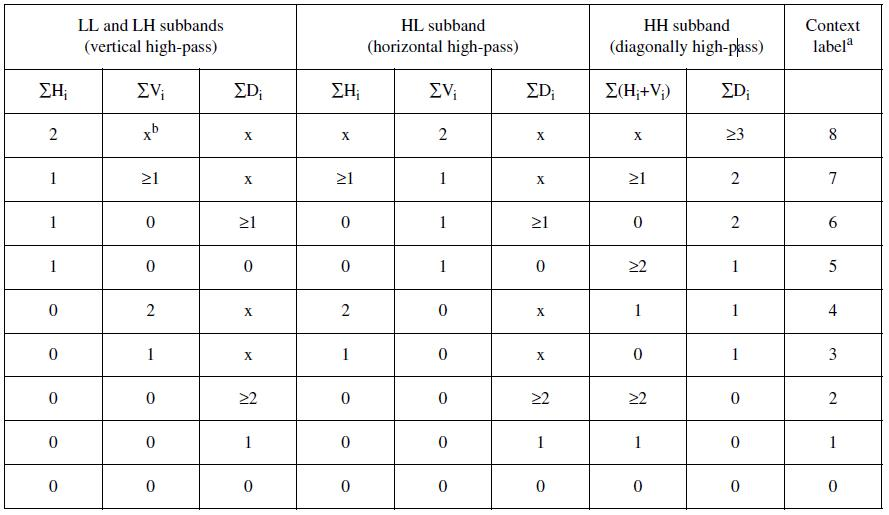
\includegraphics [width=6in]{zerocoding.jpg} 
\caption{零编码(zero coding)上下文(context)编码方式} 
\label{fig:zero coding} 
\end{figure}

\subsubsection{符号编码(Sign Coding)}
该编码根据待编码的数据比特上、下、左、右的4个相邻数据重要性情况以及待编码数据的符号位编码,返回符号编码(XORbit)和Context。具体编码规则如表{~\ref{tab:sign coding}}所示。其中“1”表示在垂直或者水平方向的相邻两个数据都为重要并且符号都为正;或者只有一个是重要的情况。“0”表示两个方向的相邻数据中两个数据都不重要或者都为重要但是具有不同的符号。-1表示的情况和1的情况相反。\textit{代码见函数SignCoding。}

\begin{table}[h]
\begin{center}
\begin{tabular}{|c|c|c|c|}
\hline
\textbf{Horizontal contribution} & \textbf{Vertical contribution} & \textbf{Context label} & \textbf{XORbit}\\
\hline
1 & 1 & 13 & 0\\
\hline
1 & 0 & 12 & 0\\
\hline
1 & -1 & 11 & 0\\
\hline
0 & 1 & 10 & 0\\
\hline
0 & 0 & 9 & 0\\
\hline
0 & -1 & 10 & 1\\
\hline
-1 & 1 & 11 & 1\\
\hline
-1 & 0 & 12 & 1\\
\hline
-1 & -1 & 13 & 1\\
\hline
\end{tabular}
\end{center}
\caption{符号编码(XORbit)和上下文(context)编码方式}
\label{tab:sign coding}
\end{table}

\subsubsection{幅度精炼编码(Magnitude Refinement Coding)}
根据该数据位是否被第一次精炼,以及$\sum H_i +  \sum V_i + \sum D_i$的值进行编码,返回D和Context。D为X的值,Context的编码规则如表{~\ref{tab:magnitude coding}}所示。\textit{代码见函数MagnitudeRefinementCoding。}

\begin{table}[h]
\begin{center}
\begin{tabular}{|c|c|c|}
\hline
\textbf{是否第一次幅度精炼编码}&\textbf{$\sum H_i +  \sum V_i + \sum D_i$}&\textbf{Context}\\
\hline
否&x&16\\
\hline
是&$\geq 1$ &15\\
\hline
是& 0 &14\\
\hline
\end{tabular}
\end{center}
\caption{幅度精炼编码(Magnitude Refinement Coding)上下文(context)编码方式}
\label{tab:magnitude coding}
\end{table}

\subsubsection{游程编码(Run Length Coding)}
仅当一个编码列(4个比特数据)的目前状态都为不重要,且相邻元素也都为不重要时,开始进行游程编码处理。这时,如果一列中的4个数据也为不重要数据,则统一编码为一个上下文编码CX=17和编码数据D=0。如果4个数据中至少有一个变为重要,则首先将其表示一个上下文CX=17和编码数据D=1。然后,编码4个数据中的第一个重要数据的位置信息(00~11)作为D,并编码上下文为CX=18。此后,编码第一个重要数据的符号位,之后数据的编码按照零编码算法进行。具体编码规则如表{~\ref{tab:runlength coding}}所示。\textit{代码见函数RunLengthCoding。}

\begin{table}[h]
\begin{center}
\begin{tabular}{|c|c|c|}
\hline
\textbf{4个比特数据}&\textbf{D}&\textbf{Context}\\
\hline
(0,0,0,0)&[0]&[17]\\
\hline
(1,x,x,x)&[1,0,0] + 符号编码+零编码 &[17,18,18]+ 符号编码+零编码\\
\hline
(0,1,x,x)&[1,0,1] + 符号编码+零编码 &[17,18,18]+ 符号编码+零编码\\
\hline
(0,0,1,x)&[1,1,0] + 符号编码+零编码 &[17,18,18]+ 符号编码+零编码\\
\hline
(0,0,0,1)&[1,1,1] + 符号编码&[17,18,18]+ 符号编码\\
\hline
\end{tabular}
\end{center}
\caption{游程编码(Run Length Coding)D和上下文(context)编码方式}
\label{tab:runlength coding}
\end{table}

\subsection{分流通道}
\subsubsection{重要性传播编码通道}
在此通道中,编码位平面中的目前状态为“无效态”,但有很大概率成为“有效态”的比特数
据。只要四周的8个比特数据有一个是重要的,就将被进行零编码(Zero Coding)。在此基础上,如果该位的比特数为1,再进行符号编码。流程图如图{~\ref{fig:twopasses}}所示。\textit{代码见函数SignifiancePropagationPass。}

\begin{figure}[h]
\centering  
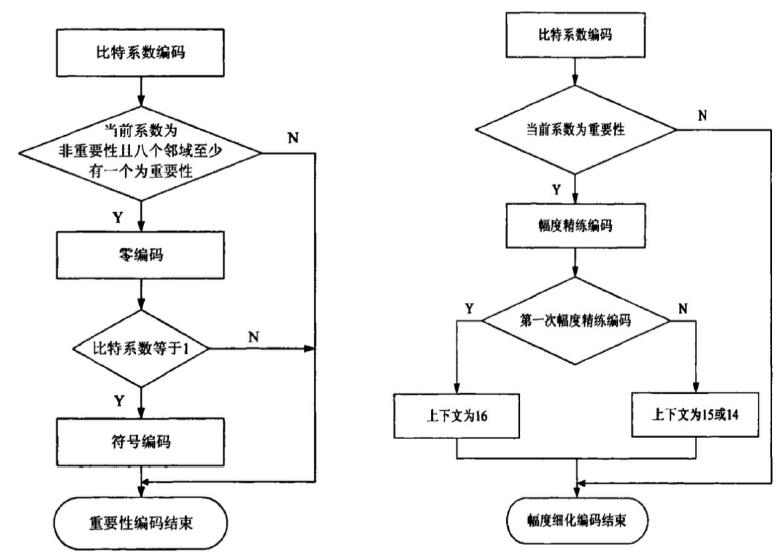
\includegraphics [width=6in]{twopasses.jpg} 
\caption{重要性传播编码通道(左)及幅度精炼编码通道(右)编码流程图} 
\label{fig:twopasses} 
\end{figure}

\subsubsection{幅度精炼编码通道}
在此通道中,编码那些在先前位平面己经被判定为有效态的数据,用“幅度精炼编码”编码。流程图如图{~\ref{fig:twopasses}}所示。\textit{代码见函数MagnitudeRefinementPass。}

\subsubsection{清除编码通道}
在此通道中,编码位平面中所有还未编码的数据。当一列4个比特都在此通道中被编码,且这4个比特都没有重要的相邻数据,则对4个比特采用游程编码(RLC),否则分别对每个比特采用零编码(Zero Coding),如数据为1,再进行符号编码(Sign Coding)。流程图如图{~\ref{fig:cleanpass}}所示。\textit{代码见函数CLeanUpPass。}

\begin{figure}[h]
\centering  
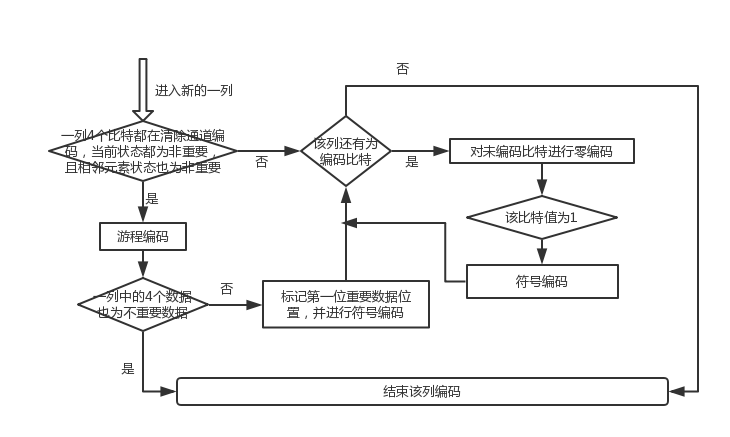
\includegraphics [width=6in]{cleanpass.jpg} 
\caption{清除编码通道编码流程图} 
\label{fig:cleanpass} 
\end{figure}

\subsection{编码流程}
\subsubsection{区段分块}
将上一步量化后的频块进一步切成32×32的区段,作为内嵌区段编码的对象,各区段之间独立运算。如频块不能被32整除,则用0补足。//
\textit{问题:用0补足时是否会增加编码的冗余?}

\subsubsection{位元层及符号矩阵}
对把编码区段内的数据取绝对值,依照位元深度,从高位元(MSB)到低位元(LSB)分成数个位元层。(\textit{量化后的数据范围是XX–XX,故共有X位})此外,由数据的正负组成符号矩阵,其中0表示正数,1表示负数。

\subsubsection{初始化上下文、重要性等矩阵}
在对整个区段编码的过程中,需要用到的矩阵及其含义如表{~\ref{tab:matrixForCoding}}所示。
\begin{table}[h]
\begin{center}
\begin{tabular}{|c|c|c|}
\hline
\textbf{矩阵(向量)名称}&\textbf{大小}&\textbf{含义}\\
\hline
重要性矩阵(S1)&32*32&表明当前状态是否为重要(用于零编码及游程编码)\\
\hline
精炼标记矩阵(S2)& 32*32 & 表明该元素是否被精炼(用于精炼编码)\\
\hline
编码标记矩阵(S3)& 32*32 & 表明该元素是否被编码(用于精炼通道及清除编码通道)\\
\hline
符号矩阵(signs)&32*32&表明该元素的符号(用于符号编码)\\
\hline
位元层(bitplanes)&X*32*32 &小波变化量化后的2进制位元表示\\
\hline
D & N*1 &编码输出矩阵\\
\hline
上下文(CX)& N*1& 编码输出上下文矩阵\\
\hline
\end{tabular}
\end{center}
\caption{编码中使用的矩阵说明}
\label{tab:matrixForCoding}
\end{table}

\subsubsection{逐位元层编码}
由高位至低位,对各位元层编码。对于各位元层,依次按照重要性传播编码通道,幅度精炼编码通道,以及清除编码通道的顺序编码。在编码各通道时,按照如图{~\ref{fig:codeorder}}所示的方式扫描。扫描过程从位平面左上角的数据开始,以4个数据为一组,连续扫描第一列的第一组4个数据后,然后转向扫描第二列的第一组4个数据,如此一直扫描到最后一列的第一组4个数据。然后,转向扫描第一列的第二组4个数据,一直到最后一列的第二组4 个数据。按照这样的顺序依次扫描整个位平面。扫描过程中矩阵的更新情况如表{~\ref{tab:matrixUpdate}}所示。\textit{代码见函数codeBlockfun。}
\begin{figure}[h]
\centering  
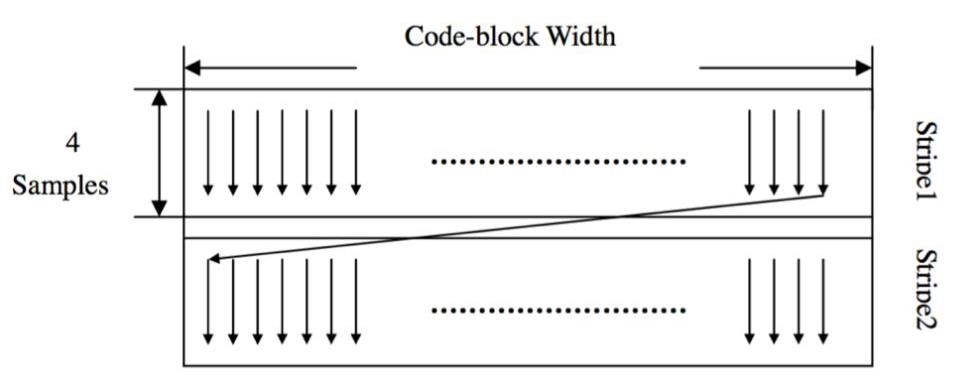
\includegraphics [width=4in]{codeorder.jpg} 
\caption{位平面扫描顺序示意图} 
\label{fig:codeorder} 
\end{figure}

\begin{table}[h]
\begin{center}
\begin{tabular}{|c|c|}
\hline
\textbf{矩阵(向量)名称}&\textbf{更新时间}\\
\hline
重要性矩阵(S1)&重要性传播编码通道及清除编码通道中更新\\
\hline
精炼标记矩阵(S2)& 精炼通道中更新\\
\hline
编码标记矩阵(S3)& 重要性传播编码通道及精炼通道中更新,结束一层位平面编码清零\\
\hline
D & 各通道都更新\\
\hline
上下文(CX)& 各通道都更新\\
\hline
\end{tabular}
\end{center}
\caption{扫描过程中矩阵的更新情况说明}
\label{tab:matrixUpdate}
\end{table}